\part{Variabili Aleatorie con Densità e Introduzione alla Statistica \\ Lezioni di Maurizio Pratelli}

\chapter{Variabili Aleatorie con densità (continue)}

\section{Svolgere integrali multipli}
\begin{defn}
    \textbf{Integrale Multiplo} \\
    Un integrale multiplo è un integrale definito di una funzione a più di una
    variabile reale. Gli integrali di una funzione $f(x,y)$ su una regione di $
    \R^2 $ sono detti \textbf{integrali doppi}, quelli di una funzione
    $f(x,y,z)$ su una regione di $ \R^3 $ sono detti \textbf{integrali tripli}.

    Proprio come l'integrale definito di una funzione positiva ad una variabile
    rappresenta l'area della regione sottostante al grafico della funzione,
    l'integrale doppio di una funzione positiva a due variabili reali
    rappresenta il volume della regione fra la superfice definita dalla funzione
    (sul piano cartesiano tridimensionale dove $ z = f(x, y)$) e il piano che
    contiene il dominio dell'integrale. Se sono presenti più variabili, un
    integrale multiplo produrrà ipervolumi di funzioni multidimensionali.
    L'integrazione multipla di una funzione ad $n$ variabili $f(x_1, x_2,
    \hdots, x_n)$ su un dominio $D$ è rappresentata da segni di integrale
    nidificati, nell'ordine inverso di esecuzione (l'integrale più a sinistra è
    calcolato per ultimo), seguita dalla funzione e i differenziali nell'ordine
    proprio (il segno di integrale più a sinistra corrisponde al differenziale
    più a destra). Il dominio di integrazione è rappresentato su ogni integrale,
    o simbolicamente abbreviato attraverso un simbolo di variabile
    sull'integrale più interno.
\end{defn}


\begin{defn}
    \textbf{Regola pratica per gli integrali doppi} \\
    \begin{equation*}
        \iint_{\R^2} f(x,y) dx dy = \int_{\R} \left( \int_{\R} f(x,y) dy \right) dx = \int_{\R} dx \int_{\R} f(x,y) dy \\
        = \int_{\R} dy \int_{\R} f(x,y) dx
    \end{equation*}
\end{defn}

\begin{exmp}
    \begin{figure}[htbp]
        \centering
        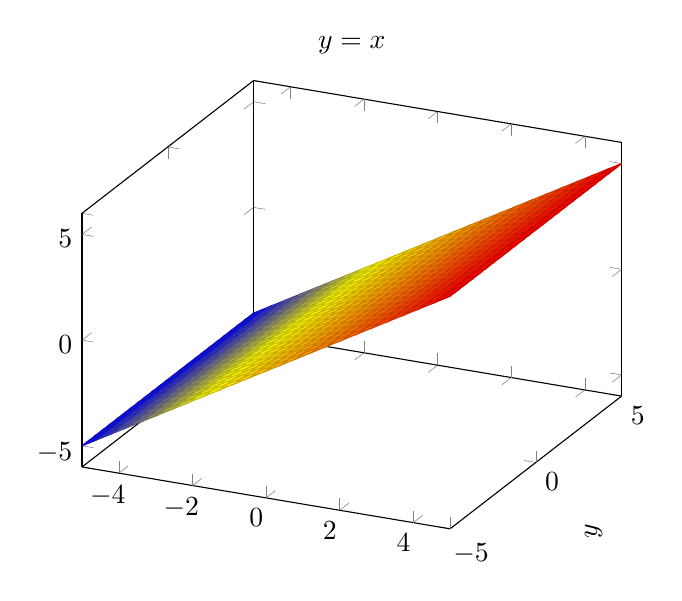
\begin{tikzpicture}
            \begin{axis}[axis lines=box, title={$y = x$},  ylabel=$y$,]
                \addplot3[surf,
                %domain=-2:2, domain y=-1.3:1.3,
            ] {x};
            \end{axis}
            \end{tikzpicture}
        \caption{Grafico della funzione $y = x$ su $\R^2$}
        \label{2varplot}
    \end{figure}
    Svolgiamo l'integrale doppio sul triangolo $ T = 0 \leq y \leq x \leq 1$ di
    $f(x,y) = x$
    \begin{equation*}
        \begin{aligned}
            \iint_T x dydx = \int_0^1 \int_0^x x dydx = \int_0^1 dx \int_0^x x dy = \int_0^1 x^2 dx = \frac{1}{3} \\
        \end{aligned}
    \end{equation*}
    Che coincide, scambiando l'ordine di integrazione con
    \begin{equation*}
        \begin{aligned}
            \int_0^1 dy \int_y^1 x dx = \frac{1}{2} \int_0^1 (1-y^2) dy = \frac{1}{2} - \frac{1}{6} = \frac{1}{3}
        \end{aligned}
    \end{equation*}

\end{exmp}

\begin{exmp}
    \begin{figure}[htbp]
        \centering
        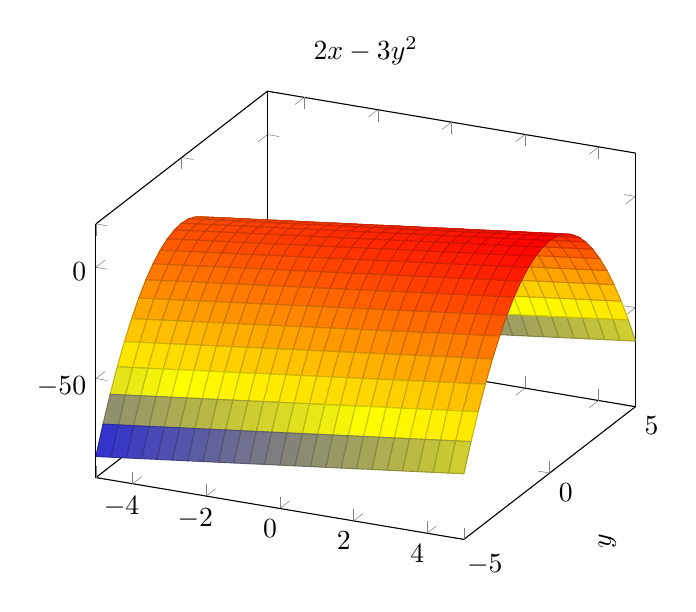
\begin{tikzpicture}
            \begin{axis}[axis lines=box, title={$2x-3y^2$},  ylabel=$y$,]
                \addplot3[surf,
                %domain=-2:2, domain y=-1.3:1.3,
            ] {2*x-3*y^2};
            \end{axis}
            \end{tikzpicture}
        \caption{Grafico della funzione reale a due variabili $2x-3y^2$}
        \label{2varplot2}
    \end{figure}
    Svolgiamo l'integrale doppio $\iint_R 2x-3y^2 dx dy$ sul rettangolo $R: -1
    \leq x \leq 1, 0 \leq y \leq 2$.

    \begin{equation*}
        \begin{aligned}
            \iint_R 2x-3y^2 dx dy = \int_0^2 \left( \int_{-1}^1 2x - 3y^2 dx \right) dy = \\
            \int_0^2 -6y^2 dy = (-6* \frac{8}{3}) = -16
        \end{aligned}
    \end{equation*}

\end{exmp}

\section{Introduzione alle Variabili Aleatorie con Densità}
\begin{defn}
    \textbf{Variabile Aleatoria}
    Abbiamo visto nella parte precedente del corso le variabili aleatorie. Una
    variabile aleatoria è una funzione definita come


    \begin{equation*}
        X: (\Omega, \mathbb{F}, P) \to \R
    \end{equation*}

    Permette di trasportare le probabilità dai sottoinsiemi di $ \Omega $ ai
    sottoinsiemi di $ \R $, ovvero


    \begin{equation*}
        \begin{aligned}
            \text{P}_X(A) = \p{X^{-1} (A)} \\
            A \subseteq \R \\
            X^{-1}(A) \subseteq \Omega
        \end{aligned}
    \end{equation*}

    Le variabili aleatorie possono essere di \textbf{discrete}, \textbf{con
    densità} o \textbf{più generali}. Una variabile aleatoria è discreta se la
    sua immagine è finita o numerabile, ovvero


    \begin{equation*}
        p(x_i) = \p{X=x_i}
    \end{equation*}
\end{defn}


\begin{defn}
    \label{defn:densita}
    \textbf{Variabile Aleatoria con Densità} \\
    $ X $ ha densità se esiste una funzione $ f : \R \to [0, +\infty) $ (la
    densità) integrabile, tale che

    \begin{equation*}
        \begin{aligned}
            \p{X \in A} = \int_A f(x)dx \\
            \p{a \leq X \leq b} = \int_a^b f(x)dx
        \end{aligned}
    \end{equation*}

    Perché $f$ sia densità una condizione necessaria è che $\int_{\Omega} f(x)
    dx = 1$, dove in generale, $\Omega = \R$ se la funzione di densità è ad una
    variabile.

    Il simbolo tilde ($\sim$) si usa per indicare che una variabile aleatoria ha una data
    distribuzione di probabilità, ad esempio $X \sim \Gamma(k, \theta)$
\end{defn}

\begin{defn}
    \textbf{Funzione di ripartizione (cumulative distribution function)} \\
    È una funzione definita come $ F : \R \to [0,1]$ È definita come
    \begin{equation*}
        F_X(x) = \p{X \leq x}
    \end{equation*}
    Se ne inferisce che la probabilità che la variabile aleatoria con densità $
    X $ risieda nell'intervallo semichiuso $(a,b]$ con $ a \leq b $ è quindi
    \begin{equation*}
        \p{a \leq X \leq b} = \p{X \leq x}
    \end{equation*}

    Sulle \textbf{variabili discrete} è tipicamente discontinua, definita come
    \begin{equation*}
        F_x(t) = \sum_{x_i \leq t} \p{X = x_i} = \sum_{x_i \leq t} p(x_i)
    \end{equation*}

    \textbf{Funzione di ripartizione su variabili con densità}
    Sulle \textbf{variabili con densità} è tipicamente continua e può essere
    espressa come l'integrale della funzione di densità di probabilità della
    variabile come segue:
    \begin{equation*}
        F_X(t) = \int_{-\infty}^{t} f(x) dx
    \end{equation*}
\end{defn}

\begin{defn}
    \textbf{Proprietà di una funzione di ripartizione} \\
    \begin{itemize}
        \item $s < t \implies F_X(1) \leq F_X(t)$ % TODO dim
        \item $\lim_{x \to -\infty} F(x) = 0$ \\
            $\lim_{x \to +\infty} F(x) = 1$
        \item $F(x) = \lim_{y \to x^+} F(y)$
    \end{itemize}
\end{defn}

\section{Proprietà principali delle variabili aleatorie con densità}

\begin{defn}
    \label{defn:indipendenzac}
    \textbf{Indipendenza di variabili con densità} \\
    La definizione di indipendenza di due variabili con densità è identica al
    caso in cui le variabili siano discrete, ma dev'essere data parlando solo di
    sottoinsiemi misurabili di $\R$. Due variabili aleatorie con densità si
    dicono tra loro indipendenti se, $\forall$ coppia $A,B$ di sottoinsiemi
    \textit{misurabili} di $\R$, risulta:
    \begin{equation*}
        \begin{aligned}
            \p{X \in A, Y \in B} = \p{X \in A}\p{Y \in B}
        \end{aligned}
    \end{equation*}

    Si osserva facilmente che due variabili aleatorie $X,Y$ sono indipendenti
    $\iff \forall$ coppia di numeri reali $s,t$, risulta

    \begin{equation*}
        \begin{aligned}
            \p{X \leq s, Y \leq T} = F_X(s)F_Y(t)
        \end{aligned}
    \end{equation*}

    Dove $F_X$ e $F_Y$ sono le rispettive funzioni di ripartizione di $X$ e $Y$.
\end{defn}


\begin{defn}
    \textbf{Assenza di memoria delle variabili aleatorie con densità
    esponenziale} \\
    \begin{equation*}
        \begin{aligned}
            \p{X > 1 + t \mid X > 1} = \p{X > t}
        \end{aligned}
    \end{equation*}

    \begin{proof}
        \begin{equation*}
            \begin{aligned}
                \p{X > t} = \p{X \in [t, +\infty]} = \int_{t}^{+\infty} \lambda e^{-\lambda x} dx \\
                = -e^{-\lambda x} \Big|_{t}^{+\infty} = e^{-\lambda t}
            \end{aligned}
        \end{equation*}
        \begin{equation*}
            \begin{aligned}
                \frac{\p{X > t + 1 \cap X > 1}}{\p{X > 1}} = \frac{e^{-\lambda (t + 1)}}{e^{-\lambda}} = e^{-\lambda t}
            \end{aligned}
        \end{equation*}
    \end{proof}
\end{defn}

\begin{defn}
    \textbf{Formula della convoluzione} \\
    La \textbf{convoluzione} è un'operazione fra due funzioni ad una variabile
    che consiste nell'integrare il prodotto tra la prima e la seconda traslata
    un certo valore. In probabilità si usa la convoluzione per ottenere la
    distribuzione di una somma di due variabili aleatorie con densità.

    \begin{equation*}
        \begin{aligned}
            (f \star g)(x) = \int_{\R}f(x - y)g(y) dy
        \end{aligned}
    \end{equation*}

    Siano date due variabili aleatorie: $X$ con densità $f(x)$ e $Y$ con densità
    $g(x)$. Sia data la coppia di v.a. $(X, Y)$ con densità $g(x)$. ne ottiene
    che:

    \begin{equation*}
        \begin{aligned}
            X \text{ ha densità } f(x) = \int_{-\infty}^{+\infty} h(x,y) dy; \>\>
            Y \text{ ha densità } g(x) = \int_{-\infty}^{+\infty} h(x,y) dx \\
        \end{aligned}
    \end{equation*}

    Se $X$ e $Y$ sono indipendenti e $Z = X + Y$ allora, la densità di $Z$ detta
    $a(z)$ sarà data dalla formula di convoluzione:

    \begin{equation*}
        \begin{aligned}
            a(z) = (g \star f)(z) = \int_{-\infty}^{+\infty} f(x) g(z-x) dx = (f \star g)(z) = \int_{-\infty}^{+\infty} g(y) f(z-y) dy
        \end{aligned}
    \end{equation*}

    Viene rispettata la commutatività della somma.

    \begin{proof}
        \begin{equation*}
            \begin{aligned}
                \p{X \leq x} = \p{X \leq x, -\infty \leq Y \leq +\infty}
            \end{aligned}
        \end{equation*}
        La variabile $Y$ è libera mentre la $X$ è limitata dal valore di $x$. Ne
        segue che:

        \begin{equation*}
            \begin{aligned}
                \p{X \leq x, -\infty \leq Y \leq +\infty} = \int_{-\infty}^{x} \int h(t, y) dy dt \\
                f(x) = \frac{d}{dx} \int_{-\infty}^{x} \int h(t, y) dy dt = \int_{-\infty}^{+\infty} h(x,y) dy
            \end{aligned}
        \end{equation*}

        Per quanto riguarda $Z = X + Y$ si ha che:

        \begin{equation*}
            \begin{aligned}
                \p{X + Y \leq Z} = \int_{-\infty}^{+\infty} f(x) \left( \int_{-\infty}^{z - x} g(y) dy \right) dx = A(z) \\
                a(z) = \int_{-\infty}^{+\infty} f(x) g(z - x) dx
            \end{aligned}
        \end{equation*}
    \end{proof}
\end{defn}

\begin{defn}
    \textbf{Prodotto di variabili aleatorie con densità a valori positivi} \\
    Siano date $X$ e $Y$ variabili aleatorie con corrispondenti densità $f(x)$ e
    $g(y)$ a valori positivi e sia $Z = XY$ il prodotto di esse. Per calcolare
    la densità $a(z)$ di $Z$, si calcola prima la funzione di ripartizione $A(z)$.

    \begin{equation*}
        \begin{aligned}
            f(x) = \begin{cases}
                0 & x \leq 0 \\
                \text{qualche valore} & x > 0
            \end{cases} \\
            g(y) = \begin{cases}
                0 & y \leq 0 \\
                \text{qualche valore} & y > 0
            \end{cases} \\
            A(z) = \p{Z \leq z} = \begin{cases}
                0 & z \leq 0 \\
                \text{qualche valore} & z > 0
            \end{cases}
        \end{aligned}
    \end{equation*}

    La definizione precedente di $A(z)$ ha senso perché $X$ e $Y$ assumono
    valori positivi. Altrimenti, avrei dovuto distinguere il caso $z \leq 0
    \implies \p{Z \geq z} = 1 - A(z)$. Si ha quindi che (per $z > 0$)
    \begin{equation*}
        \begin{aligned}
            A(z) = \p{XY \leq z} = \int_{0}^{+\infty} dx \int_{0}^{\dfrac{z}{x}} f(x) g(y) dx
        \end{aligned}
    \end{equation*}

    Si nota che $z$ compare in questo integrale. Deriviamo adesso $G(z)$

    \begin{equation*}
        \begin{aligned}
            g(z) = \frac{d G(z)}{dz} = \int_{0}^{+\infty} \frac{1}{x} f(x) g(\frac{z}{x}) dy
        \end{aligned}
    \end{equation*}
\end{defn}


\begin{defn}
    \textbf{Speranza di variabili aleatorie con densità} \\
    Si dice che $X$ ha speranza matematica finita (o valore atteso) se
    \begin{equation*}
        \begin{aligned}
            \int_{-\infty}^{+\infty} \abs{x} f(x) dx < +\infty
        \end{aligned}
    \end{equation*}
    E si dice \textbf{speranza matematica} di $X$ il numero
    \begin{equation*}
        \begin{aligned}
            \E{X} = \int_{-\infty}^{+\infty} x f(x) dx
        \end{aligned}
    \end{equation*}
\end{defn}

\begin{defn}
    \textbf{Momenti di una variabile aleatoria con densità} \\
    Il momento $k$-esimo di una v.a. con densità, se finito, è dato da

    \begin{equation*}
        \begin{aligned}
            \E{X^k} = \int_{-\infty}^{+\infty} x^k f(x) dx \\
            \exists \E{X^k} \implies \exists \E{X^m} & 1 \leq m < k
        \end{aligned}
    \end{equation*}
\end{defn}


\begin{defn}
    \textbf{Proprietà della speranza} \\
    \begin{itemize}
        \item \textbf{Regola della somma (linearità)}:
        \begin{equation*}
            \begin{aligned}
                \E{X + Y} = \E{X} + \E{Y} \\
                \E{\alpha X} = \alpha \E{X}
            \end{aligned}
        \end{equation*}
        \item \textbf{Regola del prodotto}: Se $X$ e $Y$ sono indipendenti allora
        \begin{equation*}
            \begin{aligned}
                \E{XY} = \E{X} \E{Y}
            \end{aligned}
        \end{equation*}
        \item \textbf{Monotonia}:
            \begin{equation*}
                \begin{aligned}
                    X \geq 0 \land \E{X} \geq 0 \land X \leq Y \implies \E{X} < \E{Y}
                \end{aligned}
            \end{equation*}
    \end{itemize}

    \begin{proof}
        Dimostriamo la monotonia del valore atteso di una variabile aleatoria
        con densità che assume solo valori positivi:
        \begin{equation*}
            \begin{aligned}
                X \geq 0 \implies f(x) = \begin{cases}
                    0 & x \leq 0 \\
                    \text{qualche valore} & x > 0
                \end{cases} \implies \exists \E{X} \\
                \E{X} = \int_{-\infty}^{0} x f(x) dx + t_{0}^{+\infty} x f(x) dx \geq 0
            \end{aligned}
        \end{equation*}
    \end{proof}
    
\end{defn}

\begin{defn}
    \textbf{Varianza di una variabile aleatoria con densità} \\
    Se $X$ ha momento secondo ($\E{X^2}$) finito, allora si definisce, come nel
    caso discreto, la varianza
    \begin{equation*}
        \begin{aligned}
            \var{X} = \E{(X - \E{X})^2} = \int_{-\infty}^{+\infty} (x - \E{X})^2 f(x) dx = \\
            \E{X^2} - \E{X}^2 = \int_{-\infty}^{+\infty} x^2 f(x) dx - \left(\int_{-\infty}^{+\infty} x (x) dx\right)^2
        \end{aligned}
    \end{equation*}
\end{defn}

\begin{defn}
    \textbf{Covarianza} \\
    La covarianza è un numero che fornisce una misura di quanto due variabili
    aleatorie varino insieme, ovvero della loro dipendenza:

    \begin{equation*}
        \begin{aligned}
            \covar{X,Y} = \E{(X  - \E{X})(Y - \E{Y})} = \E{XY} - \E{X}\E{Y}
        \end{aligned}
    \end{equation*}

    Due variabili aleatorie hanno covarianza $= 0$ se sono indipendenti. Si nota
    anche che

    \begin{equation*}
        \begin{aligned}
            \covar{X,X} = \var{X} \\
            \var{X + Y} = \var{X} + \var{Y} + 2\covar{X, Y}
        \end{aligned}
    \end{equation*}
\end{defn}

\begin{defn}
    \textbf{Disuguaglianze di Markov e Chebishev} \\
    Le disuguaglianze di Markov e Chebishev sono identiche nel caso due
    variabili aleatorie siano discrete o con densità. Dimostriamo la
    disuguaglianza di Markov.

    \begin{prop}
        \begin{equation*}
            \begin{aligned}
                \p{X > a} \le \dfrac{\E{X}}{a} \\
                \E{X} \geq a \p{X > a}
            \end{aligned}
        \end{equation*}
    \end{prop}

    \begin{proof}
        \begin{equation*}
            \begin{aligned}
                X \geq 0 \land a > 0 \implies \p{X > a} a < \E{X} \\
                X \geq 0 \implies f(x) = \begin{cases}
                    0 & x \leq 0 \\
                    \text{qualche valore} & x > 0
                \end{cases} \implies \exists \E{X} \\
                \E{X} = \int_{0}^{+\infty} x f(x) dx = \int_{0}^{a} x f(x) dx + \int_{a}^{+\infty} x f(x) dx \\
                \geq \int_{a}^{+\infty} x f(x) dx \geq \int_{a}^{+\infty} a f(x) dx
            \end{aligned}
        \end{equation*}

        Nell'integrale, $x$ varia fra $a$ e $+\infty$, se al posto di $x$
        sostituisco $a$, se ne ottiene una quantità minore poiché $a$ è il
        minimo valore che la variabile $x$ sulla quale integriamo assume.

        \begin{equation*}
            \begin{aligned}
                = a \int_{a}^{+\infty} f(x) dx = a \p{X > a}
            \end{aligned}
        \end{equation*}

    \end{proof}
\end{defn}
